% This is samplepaper.tex, a sample chapter demonstrating the
% LLNCS macro package for Springer Computer Science proceedings;
% Version 2.21 of 2022/01/12
%
\documentclass[runningheads]{llncs}
%
\usepackage[T1]{fontenc}
% T1 fonts will be used to generate the final print and online PDFs,
% so please use T1 fonts in your manuscript whenever possible.
% Other font encondings may result in incorrect characters.
%
\usepackage{graphicx}
% Used for displaying a sample figure. If possible, figure files should
% be included in EPS format.
%
% If you use the hyperref package, please uncomment the following two lines
% to display URLs in blue roman font according to Springer's eBook style:
%\usepackage{color}
%\renewcommand\UrlFont{\color{blue}\rmfamily}
%\urlstyle{rm}
%
\usepackage{amsmath}  % Required for \text command
\usepackage{amssymb}
\begin{document}
%
\title{Contribution Title}
%
%\titlerunning{Abbreviated paper title}
% If the paper title is too long for the running head, you can set
% an abbreviated paper title here
%
\author{Anna Vitali\inst{1}\orcidID{0000-1111-2222-3333} \and
Second Author\inst{2,3}\orcidID{1111-2222-3333-4444} \and
Third Author\inst{1}\orcidID{2222--3333-4444-5555}}
%
\authorrunning{A. Vitali, R. Amadini et al.}
% First names are abbreviated in the running head.
% If there are more than two authors, 'et al.' is used.
%
\institute{Alma Mater Studiorum Università di Bologna, Bolgona, Italy\\
%\url{http://www.springer.com/gp/computer-science/lncs} \and
%ABC Institute, Rupert-Karls-University Heidelberg, Heidelberg, Germany\\
\email{\{anna.vitali7\}@unibo.it}}
%
\maketitle              % typeset the header of the contribution
%
\begin{abstract}
The abstract should briefly summarize the contents of the paper in
150--250 words.

\keywords{First keyword  \and Second keyword \and Another keyword.}
\end{abstract}
%
%
%

\section{Introduction}

In manufacturing industry, finding the correct positioning of the parts fasteners during the milling and cutting processes, in order to reduce vibrations and keep the element as firm as possible, is a fundamental problem to be solved to ensure a certain quality of the finished product \cite{fei2020state}.

Several studies have been carried out on the forms and materials that can be used to minimize oscillations and vibrations \cite{sivasubramanian2019optimization,chung2001materials}, among these one of the most adopted strategies in the manufacturing field involves the use of adsorption methods based on the adoption of vacuum suction cups \cite{zhu2006principle,del2019thin}.

In this study, we will use as a reference a machine capable of performing operations on a wooden panel, such as milling, contouring, and drilling, supported by a system of movable bars on which suction cups can be vertically adjusted for secure holding. 

Several factors must be taken into account for effective positioning of suction cups, including the type of machining operation, the specific areas of the workpiece that will be affected, and the geometry of the part \cite{rachierumethodology}. In particular, when dealing with cutting operations, it is essential to avoid placing fixtures beneath areas where through-cuts will occur to prevent potential damage to the fasteners.

It is also important to consider that the available resources are limited. Typically, the machine has a fixed capacity, allowing for only a certain number of bars and a finite number of various types of fixings. Within these constraints, we must decide how to allocate the resources efficiently, ensuring that we do not exceed the available quantity while providing adequate support for the workpiece. The objective, however, is not to maximize the use of resources but to strategically cover the most critical areas of the workpiece to achieve optimal support.

To address this problem, we propose a constraint optimization model to decide where to place the bars and on them where the suction cups can be inserted and we compered the results with those generated by the current system. The comparison revealed that the solution obtained via CP was easier to implement, reducing the risk of human error. Indeed, in the current system, the machine operator must manually specify the number of suction cups to be used, which increases the likelihood of errors, especially when too few are selected.

Moreover, the CP-based solution demonstrated an improvement in the support of the workpiece. Specifically, the solution ensures that if components are cut from the original piece, each sub-part large enough to accommodate suction cups is adequately supported, thereby preventing its unintended detachment. This is achieved by ensuring that the center of gravity of each sub-part remains within the perimeter formed by the fixtures inside it. In contrast, examples show that some solutions generated by the current system fail to meet this requirement, whereas the CP solution consistently satisfies this condition.

The remainder of this article is organized as follows. Section 2 presents an overview of similar problems that have been addressed using Constraint Programming. In Section 3, we explain the method used to identify the optimal points for support placement and how these points are represented. Section 4 details the constraint model developed to determine the positioning of the elements. Finally, Section 5 presents the results of our approach, comparing them with those of the previous system.

\section{Related works}

\section{Identification of Optimal Fastener Placement Points}

\section{Model}
In this section, we delineate the fundamental components of our model, including the input parameters, variables, constraints, and objective function. The model is characterized as \textit{parametric} because the definitions of the variables, constraints, and objective function are contingent upon the input parameters.

\subsection{Parameters}
The input parameters are those \textit{constant} values shaping a particular \textit{instance} of the model \cite{wallace2020building}. We formalize them as follows.

\subsubsection{Capacity, Resources and Position}
We define \(\mathsf{capacity}\) as the total space available along the reference axis for the placement of bar or suction cup devices. Additionally \(\mathsf{max\_resources}\) represents the maximum number of bar or suction cups that can be utilized by the machine, while \(\mathsf{max\_position}\) indicates the maximum number of locations available for device insertion. 

We assume that all these values are integers, determined based on the geometry of the workpiece and the resources allocated to the machine. 

The placement of objects must be arranged in such a manner that they do not overlap with one another and do not exceed the available capacity.


\subsubsection{Object and Positions}
Let \(\mathsf{OBJECT} = \{1, \dots,  \mathsf{max\_position}\}\) be the set of objects, and \(\mathsf{POSITIONS} = \{1, \dots, \mathsf{max\_positions}\}\) be the set of available positions. The size of each object \(i \in \mathsf{OBJECT}\) is given by the function \\\(\mathsf{object\_size} \colon \mathsf{OBJECT} \to \mathbb{N},\) where \(\mathsf{object\_size\_in\_x}[i]\) denotes the size of object \(i\). 

The profit of each position \(j \in \mathsf{POSITION}\) is defined by the function \\\(\mathsf{position\_profit} \colon \mathsf{Position} \to \mathbb{N}\) where \(\mathsf{position\_profit}[j]\) indicates the profit associated with the position \(j\).

The goal of the model is to maximize the total profit resulting form locating objects in the available positions.

\subsection{Variables}

We define the model's primary variable, \(\mathsf{object\_position}[i]\), which indicates the placement of object \(i\) on the axis of interest, where \(\mathsf{object\_position}[i] \in \mathsf{POSITION}\). Each object is either selected or not selected for placement. The selection of object \(i\) is represented by a binary variable \(\mathsf{object\_selected}[i] \in \{0, 1\}\), defined as:

\[
\mathsf{object\_selected}[i] =
\begin{cases}
	1, & \text{if object } i \text{ is selected}, \\
	0, & \text{if object } i \text{ is not selected}.
\end{cases}
\]

This approach allows us to know the number of resources that will be used and for each of them what will be its placement in the workplane, leaving out the resources that will not be allocated.

\subsection{Constraint and Objective}

The idea of Constraint Programming is to solve problems by stating constraints about the problem, and consequently, finding solution satisfying all the constraints. A \textit{constraint} is simply a logical relation among variables, restricting the possible values which they can take \cite{bartak1999constraint}. For our problem we defined the following constraints.

\subsubsection{Capacity Constraint} First of all we need to ensure that the total space occupied by the selected objects does not exceed the available \(\mathsf{capacity}\). This is formalized by the constraint

\[
\sum_{i \in \mathsf{OBJECT}} \mathsf{object\_size\_in\_x}[i] \cdot \mathsf{selected}[i] \leq \mathsf{capacity}
\]

\subsubsection{Non-overlapping Constraint} To avoid overlapping objects, we ensures that the space occupied by the \(i-th\) object, which is specified by \(\mathsf{position\_object}[i]\), if selected does not occupy the position of the next object indicated by \(\mathsf{object\_position}[x + 1]\). This is written as:

\[
(\mathsf{object\_x}[i] + \mathsf{object\_size\_in\_x}[i]) \cdot \mathsf{selected}[i] < \mathsf{object\_x}[i+1] \quad \forall i \in \mathsf{OBJECT}
\]

\subsubsection{Increasing Order Constraint} The increasing order constraint ensures that the positions of the selected objects are in strictly increasing order. This constraint is of interest to obtain the coordinates of elements in ascending order, for correctly represent them later in post-processing, and is captured by the built-in \(increasing\) constraint:

\[increasing(\mathsf{object\_position})\]

\subsection{Objective Function}

The objective function is designed to maximize the profit generated from the strategic positioning of devices. The selected object (\(\mathsf{object\_selected}\)) are positioned in specific locations (\(\mathsf{object\_position}\)), each associated with a known profit (\(\mathsf{position\_profit}\)), as a result the objective function becomes:

\[
\max \sum_{i \in \mathsf{OBJECT}} \mathsf{position\_profit}[\mathsf{object\_x}[i]] \cdot \mathsf{selected}[i]
\]

This function ensures that only the selected objects contribute to the overall profit, with the profit being contingent upon their respective placement positions.

\section{Result analysis}

\section{Conclusion}

\section{First Section}
\subsection{A Subsection Sample}
Please note that the first paragraph of a section or subsection is
not indented. The first paragraph that follows a table, figure,
equation etc. does not need an indent, either.

Subsequent paragraphs, however, are indented.

\subsubsection{Sample Heading (Third Level)} Only two levels of
headings should be numbered. Lower level headings remain unnumbered;
they are formatted as run-in headings.

\paragraph{Sample Heading (Fourth Level)}
The contribution should contain no more than four levels of
headings. Table~\ref{tab1} gives a summary of all heading levels.

\begin{table}
\caption{Table captions should be placed above the
tables.}\label{tab1}
\begin{tabular}{|l|l|l|}
\hline
Heading level &  Example & Font size and style\\
\hline
Title (centered) &  {\Large\bfseries Lecture Notes} & 14 point, bold\\
1st-level heading &  {\large\bfseries 1 Introduction} & 12 point, bold\\
2nd-level heading & {\bfseries 2.1 Printing Area} & 10 point, bold\\
3rd-level heading & {\bfseries Run-in Heading in Bold.} Text follows & 10 point, bold\\
4th-level heading & {\itshape Lowest Level Heading.} Text follows & 10 point, italic\\
\hline
\end{tabular}
\end{table}


\noindent Displayed equations are centered and set on a separate
line.
\begin{equation}
x + y = z
\end{equation}
Please try to avoid rasterized images for line-art diagrams and
schemas. Whenever possible, use vector graphics instead (see
Fig.~\ref{fig1}).

\begin{figure}
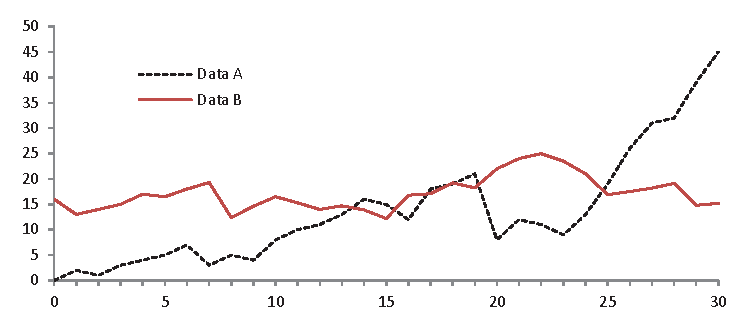
\includegraphics[width=\textwidth]{fig1.eps}
\caption{A figure caption is always placed below the illustration.
Please note that short captions are centered, while long ones are
justified by the macro package automatically.} \label{fig1}
\end{figure}

\begin{theorem}
This is a sample theorem. The run-in heading is set in bold, while
the following text appears in italics. Definitions, lemmas,
propositions, and corollaries are styled the same way.
\end{theorem}
%
% the environments 'definition', 'lemma', 'proposition', 'corollary',
% 'remark', and 'example' are defined in the LLNCS documentclass as well.
%
\begin{proof}
Proofs, examples, and remarks have the initial word in italics,
while the following text appears in normal font.
\end{proof}
For citations of references, we prefer the use of square brackets
and consecutive numbers. Citations using labels or the author/year
convention are also acceptable. The following bibliography provides
a sample reference list with entries for journal
articles~\cite{ref_article1}, an LNCS chapter~\cite{ref_lncs1}, a
book~\cite{ref_book1}, proceedings without editors~\cite{ref_proc1},
and a homepage~\cite{ref_url1}. Multiple citations are grouped
\cite{ref_article1,ref_lncs1,ref_book1},
\cite{ref_article1,ref_book1,ref_proc1,ref_url1}.

\begin{credits}
\subsubsection{\ackname} A bold run-in heading in small font size at the end of the paper is
used for general acknowledgments, for example: This study was funded
by X (grant number Y).

\subsubsection{\discintname}
It is now necessary to declare any competing interests or to specifically
state that the authors have no competing interests. Please place the
statement with a bold run-in heading in small font size beneath the
(optional) acknowledgments\footnote{If EquinOCS, our proceedings submission
system, is used, then the disclaimer can be provided directly in the system.},
for example: The authors have no competing interests to declare that are
relevant to the content of this article. Or: Author A has received research
grants from Company W. Author B has received a speaker honorarium from
Company X and owns stock in Company Y. Author C is a member of committee Z.
\end{credits}
%
% ---- Bibliography ----
%
% BibTeX users should specify bibliography style 'splncs04'.
% References will then be sorted and formatted in the correct style.
%
 \bibliographystyle{splncs04}
 \bibliography{bibliography}
%
% \begin{thebibliography}{8}




	
%%%%%%%%%%%%%%%%%%%%%%%%%%%%%%%%%%%%%%%%%%%%%%%%%%%%%%%%%%%%%%%	
	
%\bibitem{ref_article1}
%Author, F.: Article title. Journal \textbf{2}(5), 99--110 (2016)

%\bibitem{ref_lncs1}
%Author, F., Author, S.: Title of a proceedings paper. In: Editor,
%F., Editor, S. (eds.) CONFERENCE 2016, LNCS, vol. 9999, pp. 1--13.
%Springer, Heidelberg (2016). \doi{10.10007/1234567890}

%\bibitem{ref_book1}
%Author, F., Author, S., Author, T.: Book title. 2nd edn. Publisher,
%Location (1999)

%\bibitem{ref_proc1}
%Author, A.-B.: Contribution title. In: 9th International Proceedings
%on Proceedings, pp. 1--2. Publisher, Location (2010)

%\bibitem{ref_url1}
%LNCS Homepage, \url{http://www.springer.com/lncs}, last accessed 2023/10/25
%\end{thebibliography}
\end{document}
